\def\Lpontwo{10}
\def\lpontwo{20}
\def\Ltontwo{14}
\def\ltontwo{4}
\def\hh{25}
\def\myscale{0.07}
\def\mywidth{0.3}

\begin{subfigure}[t]{\mywidth\linewidth}

\centering
\tdplotsetmaincoords{70}{35}
\begin{tikzpicture}[scale=\myscale,tdplot_main_coords]

% Define coordinates
\coordinate(1) at (-\Lpontwo,-\Lpontwo,0);
\coordinate(2) at (\Lpontwo,-\Lpontwo,0);
\coordinate(3) at (\Lpontwo,\Lpontwo,0);
\coordinate(4) at (-\Lpontwo,\Lpontwo,0);
\coordinate(5) at (-\lpontwo,-\lpontwo,-\hh);
\coordinate(6) at (\lpontwo,-\lpontwo,-\hh);
\coordinate(7) at (\lpontwo,\lpontwo,-\hh);
\coordinate(8) at (-\lpontwo,\lpontwo,-\hh);

% Draw the shape
\draw (1) -- (2) -- (3) -- (4) -- cycle;
\draw (1) -- (5) -- (6) -- (7) -- (3);
\draw[dashed] (7) -- (8) -- (5);
\draw (2) -- (6);
\draw[dashed] (4) -- (8);

\node(Lp) at (-\Lpontwo-5,3,1) {\(L_p\)};
\node(Lp2) at (0,\Lpontwo+5,1) {\(L_p\)};
\node(lp) at (\lpontwo+5,0,-\hh-1) {\(l_p\)};
\node(lp2) at (3,-\lpontwo-6,-\hh-1) {\(l_p\)};

\end{tikzpicture}

\subcaption{}
\label{subfig:p3pfrus3d}

\end{subfigure}
~
\begin{subfigure}[t]{\mywidth\linewidth}
	
\centering
\tdplotsetmaincoords{70}{35}
\begin{tikzpicture}[scale=\myscale,tdplot_main_coords]

% Define coordinates
\coordinate(1) at (-\Ltontwo,-\Lpontwo,0);
\coordinate(2) at (\Ltontwo,-\Lpontwo,0);
\coordinate(3) at (\Ltontwo,\Lpontwo,0);
\coordinate(4) at (-\Ltontwo,\Lpontwo,0);
\coordinate(5) at (-\ltontwo,-\lpontwo,-\hh);
\coordinate(6) at (\ltontwo,-\lpontwo,-\hh);
\coordinate(7) at (\ltontwo,\lpontwo,-\hh);
\coordinate(8) at (-\ltontwo,\lpontwo,-\hh);

% Draw the shape
\draw (1) -- (2) -- (3) -- (4) -- cycle;
\draw (1) -- (5) -- (6) -- (7) -- (3);
\draw[dashed] (7) -- (8) -- (5);
\draw (2) -- (6);
\draw[dashed] (4) -- (8);

\node(Lp) at (-\Ltontwo-5,3,1) {\(L_p\)};
\node(Lt) at (0,\Lpontwo+5,1) {\(L_t\)};
\node(lp) at (\ltontwo+5,0,-\hh-1) {\(l_p\)};
\node(lt) at (3,-\lpontwo-6,-\hh-1) {\(l_t\)};

\end{tikzpicture}

\subcaption{}
\label{subfig:p3tfrus3d}
	
\end{subfigure}
~
\begin{subfigure}[t]{\mywidth\linewidth}
	
	\centering
	\tdplotsetmaincoords{70}{35}
	\begin{tikzpicture}[scale=0.06,tdplot_main_coords]
	
	% Define coordinates of z frustum
	\coordinate(1z) at (-\Lpontwo,-\Lpontwo,0);
	\coordinate(2z) at (\Lpontwo,-\Lpontwo,0);
	\coordinate(3z) at (\Lpontwo,\Lpontwo,0);
	\coordinate(4z) at (-\Lpontwo,\Lpontwo,0);
	\coordinate(5z) at (-\lpontwo,-\lpontwo,-\hh);
	\coordinate(6z) at (\lpontwo,-\lpontwo,-\hh);
	\coordinate(7z) at (\lpontwo,\lpontwo,-\hh);
	\coordinate(8z) at (-\lpontwo,\lpontwo,-\hh);
	
	% Define coordinates of x frustum
	\coordinate(1x) at (\Lpontwo,-\Lpontwo,0);
	\coordinate(2x) at (\Lpontwo+\Ltontwo+\Ltontwo,-\Lpontwo,0);
	\coordinate(3x) at (\Lpontwo+\Ltontwo+\Ltontwo,\Lpontwo,0);
	\coordinate(4x) at (\Lpontwo,\Lpontwo,0);
	\coordinate(5x) at (\lpontwo,-\lpontwo,-\hh);
	\coordinate(6x) at (\lpontwo+\ltontwo+\ltontwo,-\lpontwo,-\hh);
	\coordinate(7x) at (\lpontwo+\ltontwo+\ltontwo,\lpontwo,-\hh);
	\coordinate(8x) at (\lpontwo,\lpontwo,-\hh);
	
	% Define coordinates of y frustum
	\coordinate(1y) at (-\Lpontwo,\Lpontwo,0);
	\coordinate(2y) at (\Lpontwo,\Lpontwo,0);
	\coordinate(3y) at (\Lpontwo,\Lpontwo+\Ltontwo+\Ltontwo,0);
	\coordinate(4y) at (-\Lpontwo,\Lpontwo+\Ltontwo+\Ltontwo,0);
	\coordinate(5y) at (-\lpontwo,\lpontwo,-\hh);
	\coordinate(6y) at (\lpontwo,\lpontwo,-\hh);
	\coordinate(7y) at (\lpontwo,\lpontwo+\ltontwo+\ltontwo,-\hh);
	\coordinate(8y) at (-\lpontwo,\lpontwo+\ltontwo+\ltontwo,-\hh);
	
	% Deal with certain lines behind objects
	\draw(3y) -- (7y);
	\filldraw[fill=white] (1x) -- (2x) -- (3x) -- (4x) -- cycle;
	\filldraw[fill=white] (2x) -- (3x) -- (7x) -- (6x) -- cycle;
	
	% Draw z frustum
	\draw (1z) -- (2z);
	\draw (3z) -- (4z) -- (1z);
	\draw (1z) -- (5z) -- (6z);
	\draw (2z) -- (6z);
	
	% Draw x frustum
	\draw (5x) -- (6x);
	
	% Draw y frustum
	\draw (2y) -- (3y) -- (4y) -- (1y);
	
	% Draw an invisible node to align left and right pictures
	\node(invis) at (0,0,-1.75*\hh) { };
	
	\end{tikzpicture}
	\subcaption{}
	\label{subfig:p3subarray3d}
	
\end{subfigure}

\begin{subfigure}[t]{\mywidth\linewidth}
	
	\centering
	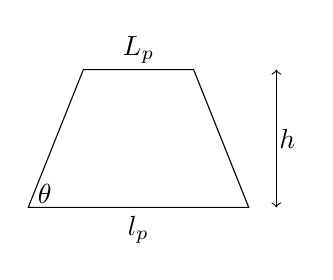
\begin{tikzpicture}[scale = \myscale]
	
	\coordinate(1) at (-\Lpontwo,0);
	\coordinate(2) at (\Lpontwo,0);
	\coordinate(5) at (-\lpontwo,-\hh);
	\coordinate(6) at (\lpontwo,-\hh);
	
	\draw (1) -- (2) -- (6) -- (5) -- cycle;
	\node(theta) at (-\lpontwo+3,-\hh+2.5) {\(\theta\)};
	\node(Lp) at (0,3.5) {\(L_p\)};
	\node(lp) at (0,-\hh-4) {\(l_p\)};
	\draw[<->] (\lpontwo+5,-\hh) -- (\lpontwo+5,0);
	\node(h) at (\lpontwo+7,-12.5) {\(h\)};
	
	\end{tikzpicture}
	
	\subcaption{}
	\label{subfig:p3pfrusschematic}
	
\end{subfigure}
~
\begin{subfigure}[t]{\mywidth\linewidth}
	
\centering
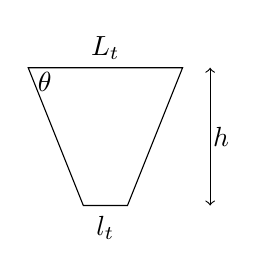
\begin{tikzpicture}[scale = \myscale]

\coordinate(1) at (-\Ltontwo,0);
\coordinate(2) at (\Ltontwo,0);
\coordinate(5) at (-\ltontwo,-\hh);
\coordinate(6) at (\ltontwo,-\hh);

\draw (1) -- (2) -- (6) -- (5) -- cycle;
\node(theta) at (-\Ltontwo+3,-2.5) {\(\theta\)};
\node(Lp) at (0,3.5) {\(L_t\)};
\node(lp) at (0,-\hh-4) {\(l_t\)};
\draw[<->] (\Ltontwo+5,-\hh) -- (\Ltontwo+5,0);
\node(h) at (\Ltontwo+7,-12.5) {\(h\)};

\end{tikzpicture}

\subcaption{}
\label{subfig:p3tfrusschematic}
	
\end{subfigure}
~
\begin{subfigure}[t]{\mywidth\linewidth}
	
	\centering
	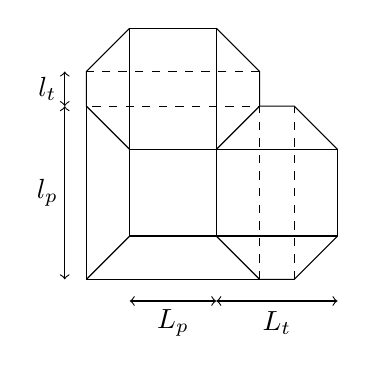
\begin{tikzpicture}[scale=0.055]
	
	% Define coordinates of z frustum
	\coordinate(1z) at (-\Lpontwo,-\Lpontwo);
	\coordinate(2z) at (\Lpontwo,-\Lpontwo);
	\coordinate(3z) at (\Lpontwo,\Lpontwo);
	\coordinate(4z) at (-\Lpontwo,\Lpontwo);
	\coordinate(5z) at (-\lpontwo,-\lpontwo);
	\coordinate(6z) at (\lpontwo,-\lpontwo);
	\coordinate(7z) at (\lpontwo,\lpontwo);
	\coordinate(8z) at (-\lpontwo,\lpontwo);
	
	% Define coordinates of x frustum
	\coordinate(1x) at (\Lpontwo,-\Lpontwo);
	\coordinate(2x) at (\Lpontwo+\Ltontwo+\Ltontwo,-\Lpontwo);
	\coordinate(3x) at (\Lpontwo+\Ltontwo+\Ltontwo,\Lpontwo);
	\coordinate(4x) at (\Lpontwo,\Lpontwo);
	\coordinate(5x) at (\lpontwo,-\lpontwo);
	\coordinate(6x) at (\lpontwo+\ltontwo+\ltontwo,-\lpontwo);
	\coordinate(7x) at (\lpontwo+\ltontwo+\ltontwo,\lpontwo);
	\coordinate(8x) at (\lpontwo,\lpontwo);
	
	% Define coordinates of y frustum
	\coordinate(1y) at (-\Lpontwo,\Lpontwo);
	\coordinate(2y) at (\Lpontwo,\Lpontwo);
	\coordinate(3y) at (\Lpontwo,\Lpontwo+\Ltontwo+\Ltontwo);
	\coordinate(4y) at (-\Lpontwo,\Lpontwo+\Ltontwo+\Ltontwo);
	\coordinate(5y) at (-\lpontwo,\lpontwo);
	\coordinate(6y) at (\lpontwo,\lpontwo);
	\coordinate(7y) at (\lpontwo,\lpontwo+\ltontwo+\ltontwo);
	\coordinate(8y) at (-\lpontwo,\lpontwo+\ltontwo+\ltontwo);
	
	% Draw top plane
	\draw (1z) -- (2z) -- (3z) -- (4z) -- cycle;
	\draw (2y) -- (3y) -- (4y) -- (1y);
	\draw (1x) -- (2x) -- (3x) -- (4x);
	
	% Draw connecting planes where necessary
	\draw (1z) -- (5z);
	\draw (1x) -- (5x) -- (6x) -- (2x);
	\draw (3x) -- (7x) -- (8x) -- (4x);
	\draw (6y) -- (7y) -- (3y);
	\draw (1y) -- (5y) -- (8y) -- (4y);
	
	% Draw bottom plane
	\draw (8z) -- (5z) -- (6z);
	\draw[dashed] (6z) -- (7z) -- (8z);
	\draw[dashed] (7y) -- (8y);
	\draw[dashed] (6x) -- (7x);
	
	% Draw some dimensions
	\draw[<->] (-\Lpontwo,-\lpontwo-5) -- (\Lpontwo,-\lpontwo-5);
	\draw[<->] (\Lpontwo,-\lpontwo-5) -- (\Lpontwo+2*\Ltontwo,-\lpontwo-5);
	\draw[<->] (-\lpontwo-5,-\lpontwo) -- (-\lpontwo-5,\lpontwo);
	\draw[<->] (-\lpontwo-5,\lpontwo) -- (-\lpontwo-5,\lpontwo+2*\ltontwo);
	\node(Lp) at (0,-\lpontwo-10) {\(L_p\)};
	\node(Lt) at (\Lpontwo+\Ltontwo,-\lpontwo-10) {\(L_t\)};
	\node(lp) at (-\lpontwo-9,0) {\(l_p\)};
	\node(lt) at (-\lpontwo-9,\lpontwo+\ltontwo) {\(l_t\)};
	
	\end{tikzpicture}
	\subcaption{}
	\label{subfig:p3subarrayschematic}
	
\end{subfigure}

